\documentclass{article}
\usepackage[preprint,nonatbib]{neurips_2025}
\usepackage[utf8]{inputenc}
\usepackage[T1]{fontenc}
\usepackage{hyperref}
\usepackage{url}
\usepackage{booktabs}
\usepackage{amsmath,amssymb}
\usepackage{microtype}
\usepackage{xcolor}
\usepackage{graphicx}
\usepackage{tikz}
\usepackage{caption}
\usepackage{enumitem}
\usetikzlibrary{positioning,arrows.meta}
\makeatletter
\renewcommand{\@noticestring}{CSE 150A/250A Final Project, Fall 2026.}
\makeatother
\captionsetup{font=small,skip=3pt}
\setlength{\textfloatsep}{9pt plus 2pt minus 2pt}
\setlength{\floatsep}{7pt plus 2pt minus 2pt}
\setlength{\abovedisplayskip}{5pt}\setlength{\belowdisplayskip}{5pt}
\setlist{nosep,leftmargin=1.3em}
\newcommand{\todo}[1]{\textcolor{red}{[#1]}}
\newcommand{\bb}{\,bb}

\title{Detecting Latent Playing Styles and Tilt in Poker\\Using Hidden Markov Models}

\author{%
  \textbf{Bob's Clan}\\
  Ishaan Tibdewal (150A) \quad Ayush Urs (250A) \quad Abhishai Ganta (150A)\\
  Pratham Chheda (250A) \quad Saksham Arora (150A)\\
  University of California San Diego
}

\newcommand{\tiltsummary}{A second HMM, in which each player is their own baseline and a shared hidden state shifts it, finds rare spells of looser play lasting about 300 hands; one starts after 3.8\% of big losses and almost never after a big win.}
\newcommand{\shiftrows}{Shift HMM, no switching, 2 / 3 states & & $-0.5847$ / $-0.5844$\\
Shift HMM, 2 states, free / input-dependent transitions & & $-0.5846$ / $-0.5846$\\}
\begin{document}
\maketitle

\begin{abstract}
Can a hidden Markov model recover playing styles from public betting actions in online poker, and does one of its states behave like \emph{tilt}, a spell of looser play after a painful loss? On 2.6 million real six-handed no-limit hold'em hands we fit HMMs with our own NumPy implementation of Baum--Welch, forward--backward and Viterbi. A four-state HMM recovers four interpretable styles (held-out players in its loose-passive state lose 7.2 big blinds per 100 hands), but they are traits, not moods: 88\% of sessions never change state. Tilt is in the raw data as a small shift (1.0 point more pots entered after a big loss than after a big win), and this HMM cannot see it. \tiltsummary
\end{abstract}

\section{Problem description}
A poker player's \emph{style} (how many hands they play, how aggressively) and their \emph{tilt} (a short period of looser, more reckless play after a painful loss) cannot be observed. What can be observed is a sequence of public betting decisions, one per hand. We ask: (1) can an HMM recover a small set of interpretable playing modes from public actions alone, and (2) does one of those modes behave like tilt, rising in probability after a large loss and decaying over the following hands?

This is a latent-variable problem with temporal structure: a mode is hidden and persists from hand to hand (a Markov chain), and the action depends on the current mode (an emission). The uncertainty is essential: three hands in four are folded whatever the mode, because the hidden cards are bad, so a mode can only be inferred by accumulating weak evidence over many hands. The question matters beyond poker. Loss-driven changes in risk taking are a classic topic in behavioural economics \cite{thaler1990}, usually studied in small laboratory samples; online poker offers millions of time-stamped decisions by real people for real money \cite{smith2009,eil2014}. Our answer to (1) is yes. Our answer to (2) is that the effect is real but small, that the proposed model is structurally unable to see it, and that a model built around that failure can.

\section{Data sourcing and processing}
\textbf{Source.} Kim's poker hand history dataset \cite{kim2024,kim2025} (mirrored as \texttt{takara-ai/poker\_hands} on Hugging Face): a scrape of no-limit hold'em cash games on six sites from July 1 to 23, 2009, giving for each hand anonymised but consistent player identifiers, stacks, every action with its bet size, the table and the start time. It also holds the 10{,}000 hands of the Pluribus bot \cite{brown2019}, our negative control.

\textbf{Filtering.} Defining a ``big loss'' needs each player's net result per hand. Winnings are complete only for PartyPoker (they are missing in 73\% of PokerStars and Full Tilt hands, 18\% of Absolute Poker, 1\% of Ongame and all of iPoker), so we use PartyPoker, at four stakes with big blinds from \$0.25 to \$10. Table size is not recorded; we keep tables with at least 200 hands at which never more than six players were dealt in: \textbf{2{,}641{,}392 hands, 331 tables, 29{,}944 players}. Amounts are in big blinds (bb). Net result is winnings minus chips put in, found by replaying the betting; it reproduces the next starting stack exactly in 90.8\% of consecutive hands (Appendix~\ref{app:data}).

\textbf{Sequences.} The proposal built one sequence per player per table. The data showed this is the wrong unit: the median session spans four tables at once. A sequence is therefore \emph{one session of one player}: all their hands at all tables in order of start time, cut where they are away for more than 30 minutes. We keep sessions of at least 100 hands and players with at least 500 such hands: \textbf{2{,}618 players, 23{,}379 sessions, 9.70M player-hands} (median session 243 hands).

\textbf{From a hand to a symbol.} Each hand contributes the player's first pre-flop decision, as two observed variables:
\begin{itemize}
\item \emph{Action} $x_t$, eight symbols: fold; check; call at a small, medium or large price; raise small, medium or large (size relative to the pot, cut at the training terciles). A three-symbol version (fold, check/call, raise) is an ablation.
\item \emph{Context} $c_t$, ten values: position group (early, cutoff, button, small blind, big blind) $\times$ whether someone has already raised. Position rotates every hand and strongly predicts the action (players fold 76\% of early-position hands but 55\% of unraised small blinds), and some symbols are impossible in some contexts (only the big blind can check). The emission is conditioned on $c_t$ so that the hidden state need not explain this.
\end{itemize}
The 4.4\% of player-hands with no decision (for example everyone folds to the big blind) stay in the sequence as \emph{missing observations} and are marginalised exactly.

\textbf{Events.} A \emph{big loss} is a hand in which the player loses at least 50\bb, half a standard buy-in; a \emph{big win} is the mirror image. (The proposal's ``50\% of the starting stack'' would count a 10\bb\ loss by a short stack.) There are 29{,}091 big losses and 33{,}527 big wins, about one hand in 300 each. Results are never an emission.

\textbf{Splits.} Players are split at random into halves. \emph{Training} data are the earliest sessions of one half, at most 2{,}000 hands per player so that high-volume players do not dominate (1{,}309 players, 1.98M hands). Held-out data are their \emph{later sessions} (2.63M hands) and all sessions of the 1{,}309 \emph{new players} (4.91M hands). Models with per-player parameters train on each player's first 70\% of hands and test on the last 30\%.

\section{Modeling and inference}
\subsection{The pooled HMM}
Each sequence $n$ has its own chain of \emph{scalar} hidden modes $z^{(n)}_t\in\{1,\dots,K\}$ and scalar symbols $x^{(n)}_t$ (Figure~\ref{fig:graph}). We do not model a table jointly: ``pooled'' means only that all sequences share one set of parameters $(\pi,A,B)$,
\begin{equation}
P(x,z\mid c)=\prod_{n=1}^{N}\Big[\pi_{z^{(n)}_1}\prod_{t=2}^{T_n}A_{z^{(n)}_{t-1}z^{(n)}_t}\prod_{t=1}^{T_n}B_{c^{(n)}_t}\big(z^{(n)}_t,x^{(n)}_t\big)\Big],
\label{eq:joint}
\end{equation}
where $B_c(k,\cdot)$ is the distribution over symbols in mode $k$ and context $c$ ($3+12+280=295$ free parameters for $K=4$). A joint model of six seats would need $K^6$ states and would answer a different question (how players react to each other).

\noindent\begin{minipage}[t]{0.53\linewidth}\vspace{0pt}
\setlength{\parindent}{0pt}\textbf{Assumptions.} (i) The mode is first-order Markov and time-homogeneous. (ii) Given mode and context the action is independent of everything else; hole cards are dealt afresh each hand, so they are emission noise, not a persistent confounder. (iii) Sequences are independent given the parameters; the main interaction between players (did someone raise before me) is routed through $c_t$. (iv) Context is not caused by the mode: position comes from the rotation, earlier raises from other players. (v) All players share the parameters, so differences \emph{between} players and changes \emph{within} a player must be expressed by the same $K$ states. Assumption (v) turns out to decide what the model learns.
\end{minipage}\hfill
\begin{minipage}[t]{0.44\linewidth}\vspace{2pt}
\centering
\resizebox{\linewidth}{!}{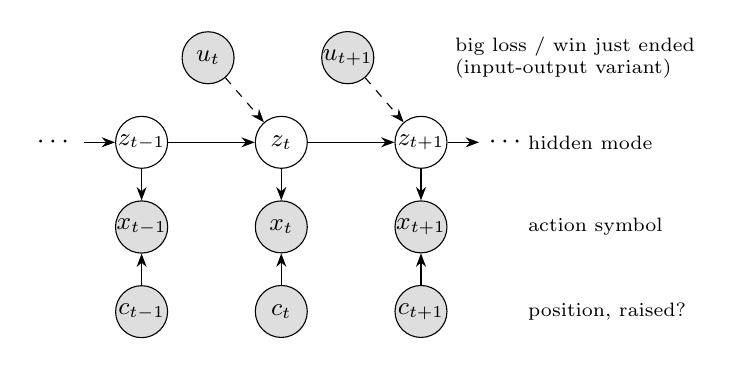
\begin{tikzpicture}[
  lat/.style={circle,draw,minimum size=6.6mm,inner sep=0pt,font=\small},
  obs/.style={lat,fill=black!13},
  >={Stealth[length=1.7mm]}, node distance=4mm and 11mm]
\node[lat] (z1) {$z_{t-1}$};
\node[lat,right=of z1] (z2) {$z_{t}$};
\node[lat,right=of z2] (z3) {$z_{t+1}$};
\node[obs,below=of z1] (x1) {$x_{t-1}$};
\node[obs,below=of z2] (x2) {$x_{t}$};
\node[obs,below=of z3] (x3) {$x_{t+1}$};
\node[obs,below=of x1] (c1) {$c_{t-1}$};
\node[obs,below=of x2] (c2) {$c_{t}$};
\node[obs,below=of x3] (c3) {$c_{t+1}$};
\node[obs,above=of z2,xshift=-9.3mm] (u2) {$u_{t}$};
\node[obs,above=of z3,xshift=-9.3mm] (u3) {$u_{t+1}$};
\node[left=4mm of z1] (d0) {$\cdots$};
\node[right=4mm of z3] (d1) {$\cdots$};
\draw[->] (d0)--(z1); \draw[->] (z1)--(z2); \draw[->] (z2)--(z3); \draw[->] (z3)--(d1);
\foreach \i in {1,2,3} {\draw[->] (z\i)--(x\i); \draw[->] (c\i)--(x\i);}
\draw[->,dashed] (u2)--(z2); \draw[->,dashed] (u3)--(z3);
\node[font=\scriptsize,anchor=west,align=left] at ([xshift=9mm]z3.east) {hidden mode};
\node[font=\scriptsize,anchor=west,align=left] at ([xshift=9mm]x3.east) {action symbol};
\node[font=\scriptsize,anchor=west,align=left] at ([xshift=9mm]c3.east) {position, raised?};
\node[font=\scriptsize,anchor=west,align=left] at ([xshift=9mm,yshift=0mm]u3.east |- u3) {big loss / win just ended\\(input-output variant)};
\end{tikzpicture}
}
\captionof{figure}{One sequence (one session of one player). Shaded nodes are observed; the dashed input $u_t$ exists only in the input-output variants.}
\label{fig:graph}
\end{minipage}

\subsection{Learning and inference}
Everything is implemented in NumPy. With $b_j(t)=B_{c_t}(j,x_t)$, or $1$ if $x_t$ is missing, the scaled recursions for one sequence are
\begin{equation}
\hat\alpha_t(j)=\frac{b_j(t)}{s_t}\sum_i\hat\alpha_{t-1}(i)A_{ij},\qquad
\hat\beta_t(i)=\frac{1}{s_{t+1}}\sum_jA_{ij}\,b_j(t+1)\,\hat\beta_{t+1}(j),
\end{equation}
with $s_t$ normalising $\hat\alpha_t$, so $\log P(x\mid c)=\sum_t\log s_t$, $\gamma_t(i)=\hat\alpha_t(i)\hat\beta_t(i)$ and $\xi_t(i,j)=\hat\alpha_{t-1}(i)A_{ij}b_j(t)\hat\beta_t(j)/s_t$. The E-step runs on each sequence separately; the M-step sums the expected counts over \emph{all} sequences and normalises \cite{rabiner1989}: $A_{ij}\propto\epsilon+\sum_{n,t}\xi^{(n)}_t(i,j)$, $B_c(i,k)\propto\epsilon+\sum_{n,t}\gamma^{(n)}_t(i)\mathbf 1[c^{(n)}_t=c,x^{(n)}_t=k]$ and $\pi_i\propto\epsilon+\sum_n\gamma^{(n)}_1(i)$.
The pseudo-count $\epsilon=0.1$ is a weak Dirichlet prior. Sequences are padded and the recursions vectorised across them (a padded step is an identity transition with emission 1); one EM iteration over 1.98M hands takes 0.42\,s on one core. Viterbi runs in log space. Emissions start at the empirical $P(x\mid c)$ times Gamma noise, transitions start sticky, and EM stops when the objective gains less than $2\times10^{-7}$ nats per decision. Each configuration is run from 5 random starts; states are then sorted by how often they fold so that state numbers are comparable across runs. \emph{Correctness}: on short sequences the likelihood, posteriors and Viterbi path equal enumeration over all $K^T$ paths to $10^{-10}$; 25 EM iterations agree with \texttt{hmmlearn} \cite{hmmlearn} to $6\times10^{-15}$; synthetic parameters are recovered (Appendix~\ref{app:impl}).

\subsection{Baselines and extensions}
\label{sec:personal}
\textbf{No hidden state} ($K=1$). \textbf{No switching} ($A=I$): one mode per session, a mixture over sessions; its gap to the HMM is what switching \emph{inside} a session is worth. \textbf{Input-output HMM} \cite{bengio1995}: $P(z_t\mid z_{t-1},u_t)=A^{(u_t)}_{z_{t-1}z_t}$, where the observed input $u_t$ marks the first hand a player starts after a big loss (or win) has ended; the M-step keeps separate transition counts per input value.

\textbf{Shift HMM.} To separate changes within a player from differences between players, we fix a baseline table $b_p(c,\cdot)$ for every player $p$ (their training counts, shrunk towards the population) and let the hidden state only \emph{shift} it:
\begin{equation}
P(x_t=k\mid z_t=j,\,c_t=c,\,\text{player }p)\;\propto\;b_p(c,k)\,e^{\theta_{jk}},\qquad\theta_{1k}=0,\quad\theta_{j,\text{fold}}=0 .
\label{eq:shift}
\end{equation}
This is a multinomial logit with a player-by-context intercept and a state effect $\theta_j$ shared by all players; state 1 is the player's own normal game. The M-step for $\theta$ is a small concave problem solved by Newton steps inside each EM iteration (generalised EM \cite{dempster1977}; Appendix~\ref{app:impl}).

\subsection{Testing for tilt}
Around every big loss we compare the 30 hands before the loss hand with the first 30 hands the player \emph{starts after it has ended} (the 6.7 hands a multi-tabler starts on average while the big pot is still being played are excluded). Two control events share the selection that the player chose to play a pot: big wins, and ``neutral flops'' (the player saw a flop and finished within $\pm10$\bb). We report the change after a loss minus the change after a control on held-out data, with 95\% intervals from 2{,}000 bootstrap resamples of \emph{players}.

\section{Results and discussion}
\subsection{How many states, and is training stable?}
\begin{figure}[t]
\centering
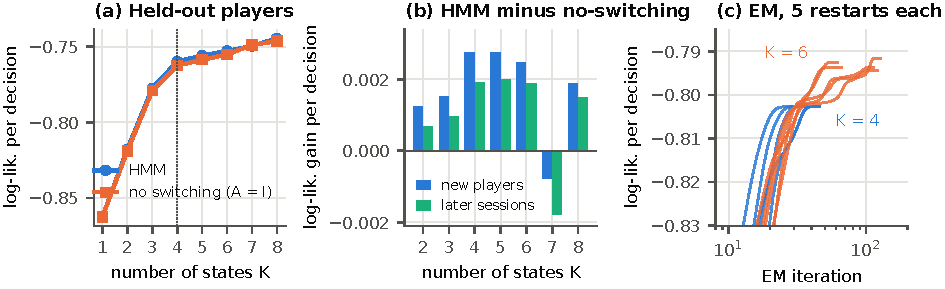
\includegraphics[width=\linewidth]{../figures/fig_selection.pdf}
\caption{(a) Held-out log-likelihood per decision against the number of states, for the HMM and for the same model with no switching. (b) Their difference. (c) Training log-likelihood during EM for five random starts each.}
\label{fig:selection}
\end{figure}
We swept $K=1,\dots,8$ (the proposal's 3 to 5, extended to see the shape). There is a clear elbow at $K=4$ (Figure~\ref{fig:selection}a; Table~\ref{tab:ll} in the appendix): on new players the log-likelihood per decision is $-0.8625$ with no hidden state, $-0.7776$ with three states, $-0.7598$ with four and $-0.7559$ with five. Held-out likelihood and BIC keep creeping up to $K=8$ (1.9 million decisions can always support a finer partition of players), so we choose $K$ by the elbow and by stability.

\textbf{Convergence.} The objective never decreased in any run. At $K=4$ all five starts reach the same optimum (to five decimals) in 32 to 46 iterations. From $K=5$ the starts end in different local optima (spread 0.003, Figure~\ref{fig:selection}c) after long plateaus, and at $K=7$ the best HMM found is worse on held-out data than the no-switching model nested inside it. Five restarts suffice at $K=4$ and not beyond.

\textbf{The uncomfortable baseline.} The no-switching model, in which a session keeps one mode throughout, reaches $-0.7626$ against the HMM's $-0.7598$. Hidden states are worth 0.103 nats per decision over $K=1$; letting the state \emph{change} within a session is worth 0.003 (Figure~\ref{fig:selection}b). Almost all the HMM learns is \emph{which kind of player this is}.

\textbf{Scalability.} Cost is linear in hands and quadratic in $K$; the whole sweep (76 fits) takes about ten minutes on 12 cores. With 295 parameters for 1.9M decisions, more data of the same kind would not change the pooled model.

\subsection{What the four states are}
\begin{figure}[t]
\centering
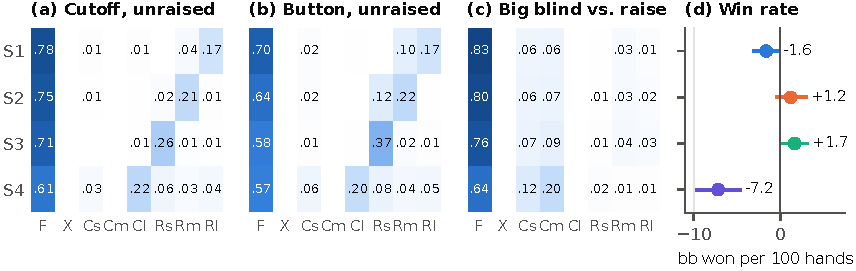
\includegraphics[width=\linewidth]{../figures/fig_states.pdf}
\caption{(a--c) Learned emission probabilities of the four states in three of the ten contexts. F fold, X check, C call and R raise at a small, medium or large size. (d) Win rate of held-out players grouped by the state they occupy most, with 95\% bootstrap intervals.}
\label{fig:states}
\end{figure}
\begin{table}[t]
\caption{The four states. Left: implied by the emission matrix (VPIP: share of hands in which money is put in voluntarily; PFR: share raised pre-flop; limp: share of unraised pots entered by calling; dwell: expected hands in the state). Right: held-out players grouped by the state they occupy most; \$0.25 is the share of their hands at the lowest stake; aggression (post-flop bets and raises per call) and win rate are never seen by the model.}
\label{tab:states}
\centering\small
\setlength{\tabcolsep}{2.6pt}
\begin{tabular}{lrrrlr|rrrr}
\toprule
 & \multicolumn{5}{c|}{Implied by emissions} & \multicolumn{4}{c}{Held-out players}\\
State (style, raise size) & VPIP & PFR & Limp & Usual raise & Dwell & Players & \$0.25 & Aggr. & Win rate, bb/100\\
\midrule
S1 tight, big & 19\% & 14\% & 3\% & large (79\%) & 1063 & 501 & 89\% & 2.6 & $-1.6$ $[-3.0,-0.3]$\\
S2 aggressive, pot-size & 23\% & 17\% & 3\% & medium (74\%) & 654 & 159 & 18\% & 2.6 & $+1.2$ $[-0.4,+2.9]$\\
S3 aggressive, small & 26\% & 20\% & 2\% & small (80\%) & 738 & 290 & 2\% & 2.7 & $+1.7$ $[+0.3,+3.1]$\\
S4 loose-passive & 37\% & 9\% & 29\% & mixed & 381 & 359 & 59\% & 1.9 & $-7.2$ $[-9.7,-4.7]$\\
\bottomrule
\end{tabular}
\end{table}
\textbf{The states match known style categories} (Figure~\ref{fig:states}, Table~\ref{tab:states}). S4 is the textbook loose-passive player: it enters 37\% of pots but raises 9\%, and limps 29\% of the time where the others limp 2 to 3\%. S1 to S3 are aggressive styles that raise nearly every pot they enter.

\textbf{They predict what the model never saw.} Held-out players who live mostly in S4 lose 7.2\bb\ per 100 hands (95\% interval $-9.7$ to $-4.7$), are the least aggressive after the flop and play the fewest hands: the recreational ``calling station''. S3 is the only group that wins after the rake.

\textbf{An unintended discovery.} S1, S2 and S3 differ mostly in the \emph{size} of their raises, and raise size is largely a convention of the game being played: 89\% of the hands of S1 players are at the \$0.25 stake and 98\% of those of S3 players at the higher stakes. The model was never told the stake and rediscovered it. A correct inference, and a warning that a fine alphabet lets states latch on to stable conventions.

\textbf{The states are traits.} Expected time in a state, $1/(1-A_{ii})$, is 381 to 1{,}063 hands, longer than the median session. On held-out players the Viterbi path changes state 0.44 times per 1{,}000 hands, 88\% of sessions have no change, and the average player spends 89\% of their hands in one state. The answer to question 1 is yes, with the qualification that the modes are styles of players, not moods.

\subsection{Is there tilt, and can an HMM see it?}
\begin{figure}[t]
\centering
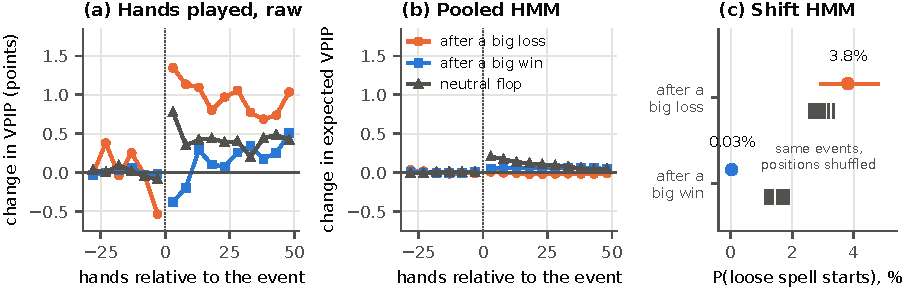
\includegraphics[width=\linewidth]{../figures/fig_tilt.pdf}
\caption{Held-out data. (a) Change in the share of hands played (VPIP) around big losses, big wins and neutral flops, relative to the player's own 30 hands before; 5-hand bins. (b) The same for the pooled HMM's posterior-expected VPIP, on the same scale. (c) Shift HMM with input-dependent transitions: probability that a loose spell starts at the first hand after an event, with 95\% bootstrap intervals; grey ticks are 20 fits with the event positions shuffled within sessions.}
\label{fig:tilt}
\end{figure}
\textbf{The raw effect is real and small.} Held-out sessions contain 13{,}957 big losses by 1{,}420 players with clean windows. In the 30 hands after a big loss players enter 1.07 points more pots than in the 30 hands before (base 22.9\%); after a big win the change is $+0.02$ and after a neutral flop $+0.46$ (Figure~\ref{fig:tilt}a). The neutral control shows that part of the rise is mechanical: the ``before'' window is required to contain no big pot, which selects quiet hands. Net of controls the loss effect is $\mathbf{+1.04}$ \textbf{points against wins} (95\% interval 0.78 to 1.31) and $+0.60$ against neutral flops (0.40 to 0.83): part loosening after losses, part tightening after wins, the ``trying to break even'' of Thaler and Johnson \cite{thaler1990} and the direction Smith et al.\ \cite{smith2009} found at high stakes. The effect is still visible 50 hands later, is larger at the lowest stake ($+1.41$ against $+0.88$) and for low-volume players, and does not depend on the threshold (Table~\ref{tab:sub}). Players also quit within 30 hands more often after a big loss (9.1\%) than after a big win (7.2\%). Across the 613 players with five or more big losses, effects vary by about 1.3 points (standard deviation) beyond sampling noise.

\textbf{The pooled HMM cannot see it.} The same event study on the pooled model's filtered posteriors is flat (Figure~\ref{fig:tilt}b); the loss-minus-win difference in posterior-expected VPIP is $-0.07$ points. This follows from assumption (v): the states are four fixed styles 3 to 18 VPIP points apart that last hundreds of hands, and a one-point shift is not a move between them. The input-output extension does not help: it raises training log-likelihood by 10.6 nats, where inputs shuffled within sessions raise it by 5.6 on average, and on held-out data it is 12 to 31 nats \emph{worse} than the plain HMM (Table~\ref{tab:io}).

\textbf{Each player as their own baseline.} If the states are busy describing who the player is, take that job away. One emission table per player with \emph{no} hidden state reaches $-0.699$ per decision on test data, against $-0.751$ for the pooled four-state HMM and $-0.736$ for eight states: knowing who is playing is worth more than any number of pooled states. A free second mode per player adds at most 0.0014 and over-fits unless a strong prior keeps the modes close (Table~\ref{tab:personal}).

\textbf{The shift HMM finds loose spells, and losses start them.} With the emissions of Eq.~(\ref{eq:shift}), two states and three symbols, EM finds a ``loose'' state with $\theta=(0.50,0.30)$ for calling and raising: odds of calling up 65\% and of raising up 35\% relative to folding, which moves an average player from playing 25.9\% of their decisions to 32.3\%. The state holds 6.9\% of test hands, starts about once in 5{,}000 hands and lasts about 300. It adds 0.0005 nats per decision on test data, 200 times less than the pooled model's hidden states, and a no-switching version with tight, normal and loose \emph{sessions} adds slightly more (0.0007): variation within a player is small and mostly between sessions. Unlike the pooled model's, this state's posterior moves the right way, rising 0.49 points more after a big loss than after a big win (0.26 to 0.72). With input-dependent transitions we obtain the estimate the proposal asked for (Figure~\ref{fig:tilt}c). The probability of entering the loose state is 0.012\% at an ordinary hand, \textbf{3.8\%} (2.9 to 4.8) at the first hand after a big loss, and 0.03\% (0.005 to 0.15) after a big win. Shuffled event positions give 2.9\% (at most 3.3\% in 20 draws) and 1.5\%, far above the ordinary rate because loose play causes big pots, so events cluster in sessions that contain spells. Against that benchmark a real loss is 1.3 times as likely to start a spell and a real win almost never does. The input does not improve held-out likelihood beyond the shuffled versions (33 nats against 30): this is an estimate of a transition probability, not a better predictor.

\textbf{Answer to question 2.} Yes in direction, no in the form we proposed. The tilt state is rare (a few percent of big losses), long (hundreds of hands, not the 20 to 50 we guessed) and accounts for at most a quarter of the average shift ($3.8\%\times6.4$ points); the rest is a diffuse change that no discrete state captures.

\textbf{Alternative explanations.} (1) \emph{Selection}: players in a loose spell are more likely to play big pots at all; the controls and the shuffled inputs share this. (2) \emph{Stack size}: a loss leaves a shorter stack at that table, which changes correct play; but for players on three or more tables most later hands are at other tables with unchanged stacks, and the effect is the same ($+1.01$). (3) \emph{Rational adjustment}: a big pot reveals information about opponents; we cannot separate deliberate adjustment from emotion, so ``tilt'' names the behavioural pattern only. (4) \emph{Who stays}: players who quit after a loss are not in the after-window, so we may under-estimate.

\subsection{Ablations and a negative control}
\label{sec:ablations}
\textbf{Context} is the most valuable modeling choice: on a common task (predicting fold, check/call or raise one step ahead; Table~\ref{tab:abl}) it improves held-out log-likelihood by 0.10 to 0.12 nats per decision, more than the hidden states do. Our stated reason for it was wrong, though: an HMM without context does not spend its states on the position cycle (decoded state and position are unrelated in every variant, Cram\'er's $V<0.01$), because sticky states cannot follow something that changes every hand. Context matters for fit, not for what the states mean. \textbf{Alphabet}: on that task the eight-symbol model predicts slightly \emph{worse} than the three-symbol one ($-0.615$ against $-0.609$); its extra symbols go to raise-size habits.

\textbf{Sequence length} (Figure~\ref{fig:ablation}a). Cutting training sessions into pieces of 5 hands lowers held-out log-likelihood by 0.016 and the learned self-transition from 0.998 to 0.970; beyond about 100 hands nothing is lost. Sequences must be long enough to accumulate evidence about a style, not to watch it change.

\textbf{Pooled or per player} (Figure~\ref{fig:ablation}b,c). With shared emissions, a transition matrix per player improves log-likelihood on later sessions from $-0.711$ to $-0.698$, best with the weakest shrinkage: it acts as a memory of the player's style. A fully personal four-state HMM matches the pooled one after about 500 of the player's own hands and beats it for 81\% of players after 1{,}000. The pooled model is right for a new player and wrong for a known one.

\textbf{Negative control} (Table~\ref{tab:pluribus}). Pluribus plays one fixed strategy, so a sound method should find no modes in its 10{,}000 hands. It finds none: a personal HMM with $K=2,3,4$ has lower cross-validated log-likelihood than $K=1$. The sobering side: the same test finds none in five of the six human professionals who played it, nor in 72\% of 40 PartyPoker players with as many hands.

\section{Conclusion}
\textbf{Findings.} (1) A four-state HMM learned from public pre-flop actions recovers playing styles that match poker's own categories and predict outcomes it never saw. (2) These states are traits: a model with no switching reaches 97\% of the HMM's gain, and the proposed tilt test on the pooled HMM finds nothing. (3) Tilt is nevertheless in the data: one point more pots entered after a big loss than after a big win. (4) An HMM in which each player is their own baseline finds rare, long spells of looser play that begin after 3.8\% of big losses and almost never after big wins.

\textbf{Limitations and extensions.} One site and three weeks in 2009; only the first pre-flop decision of each hand; no hole cards; and an observational event study, so ``after a loss'' is not ``because of a loss''. Next steps: post-flop actions as further emissions, a continuous latent style per player (a hierarchical model) in place of the fixed table, and an entry probability that depends on the size of the loss.

\section{Reflections and contributions}
\textbf{Advice for future students.} \emph{Look at the data before trusting the plan}: three facts we learned after the proposal shaped the project (winnings are missing at most sites, players sit at four tables at once, raise sizes encode the stake). \emph{Fit the dull baselines}: the no-switching model and the per-player table with no hidden state each changed what we thought the HMM was doing. \emph{Measure the effect without the model first}, and \emph{test the implementation before using it}: after agreement with enumeration and \texttt{hmmlearn}, every surprise was about the data, not a bug.

\textbf{What failed.} States did not track table position as we had predicted. Per-player modes collapsed, then over-fitted, until their prior was centred on the player's own baseline. A first shift HMM, whose loose state could only start at an event, fitted shuffled events as well as real ones (Appendix~\ref{app:more}). The input-output HMM on the pooled model was a null result.

\textbf{Contributions and individual reflections.} \todo{TEAM: at most 40 words each.}
\begin{itemize}
\item \textbf{Ishaan Tibdewal}: \todo{What I did, in one or two sentences: which parts of the project I was responsible for. Then what I personally learned from the project, in one or two sentences of my own.}
\item \textbf{Ayush Urs}: \todo{What I did, in one or two sentences: which parts of the project I was responsible for. Then what I personally learned from the project, in one or two sentences of my own.}
\item \textbf{Abhishai Ganta}: \todo{What I did, in one or two sentences: which parts of the project I was responsible for. Then what I personally learned from the project, in one or two sentences of my own.}
\item \textbf{Pratham Chheda}: \todo{What I did, in one or two sentences: which parts of the project I was responsible for. Then what I personally learned from the project, in one or two sentences of my own.}
\item \textbf{Saksham Arora}: \todo{What I did, in one or two sentences: which parts of the project I was responsible for. Then what I personally learned from the project, in one or two sentences of my own.}
\end{itemize}

\textbf{Use of generative AI.} \todo{TEAM: review and edit so that it is accurate.} We used Claude (Anthropic), through the Claude Code tool, throughout this project. It wrote the data pipeline, the NumPy HMM implementation and its tests, and the experiment and plotting scripts; it ran the experiments; and it produced the first draft of this report, including the figures. The problem, the dataset and the proposal are ours. \todo{State what the team checked, changed and wrote.}

\begin{thebibliography}{99}
\small
\bibitem{kim2024} J.~Kim. Recording and describing poker hands. In \emph{IEEE Conference on Games (CoG)}, 2024. arXiv:2312.11753.
\bibitem{kim2025} J.~Kim. A dataset of poker hand histories (v3). Zenodo, 2025. doi:10.5281/zenodo.10796885. Mirrored as \texttt{takara-ai/poker\_hands} on Hugging Face (CC BY 4.0).
\bibitem{brown2019} N.~Brown and T.~Sandholm. Superhuman AI for multiplayer poker. \emph{Science}, 365(6456):885--890, 2019.
\bibitem{rabiner1989} L.~R.~Rabiner. A tutorial on hidden Markov models and selected applications in speech recognition. \emph{Proceedings of the IEEE}, 77(2):257--286, 1989.
\bibitem{dempster1977} A.~P.~Dempster, N.~M.~Laird and D.~B.~Rubin. Maximum likelihood from incomplete data via the EM algorithm. \emph{Journal of the Royal Statistical Society B}, 39(1):1--38, 1977.
\bibitem{bengio1995} Y.~Bengio and P.~Frasconi. An input output HMM architecture. In \emph{Advances in Neural Information Processing Systems 7}, 1995.
\bibitem{smith2009} G.~Smith, M.~Levere and R.~Kurtzman. Poker player behavior after big wins and big losses. \emph{Management Science}, 55(9):1547--1555, 2009.
\bibitem{eil2014} D.~Eil and J.~W.~Lien. Staying ahead and getting even: Risk attitudes of experienced poker players. \emph{Games and Economic Behavior}, 87:50--69, 2014.
\bibitem{thaler1990} R.~H.~Thaler and E.~J.~Johnson. Gambling with the house money and trying to break even: The effects of prior outcomes on risky choice. \emph{Management Science}, 36(6):643--660, 1990.
\bibitem{hmmlearn} hmmlearn developers. hmmlearn: hidden Markov models in Python (version 0.3.3). \url{https://github.com/hmmlearn/hmmlearn}.
\bibitem{numpy} C.~R.~Harris et al. Array programming with NumPy. \emph{Nature}, 585:357--362, 2020.
\end{thebibliography}


\clearpage
\appendix
\section{Data details}
\label{app:data}
\textbf{Hands per stake} (6-max PartyPoker tables kept): 1{,}338{,}547 at \$0.10/\$0.25, 659{,}208 at \$2/\$4, 278{,}612 at \$3/\$6 and 365{,}025 at \$5/\$10. Six players are dealt in for 46\% of hands, five for 35\%, four for 13\%, three or fewer for 6\%.

\textbf{Net-result check.} For 13.3M pairs of consecutive hands of a player at one table, the next starting stack equals stack plus computed net result to within 0.02\bb\ in 90.8\% of pairs. It is higher in 6.9\% (top-ups and re-buys) and lower in 2.4\%; the lower cases follow longer time gaps (median 75\,s against 32\,s), consistent with hands missing from the scrape. Net results of a hand sum to $-0.44$\bb\ on average, the rake.

\textbf{Sessions.} Among sessions of at least 100 hands, the median session lasts 94 minutes, covers 4 tables and runs at 142 hands per hour; only 17\% are played at a single table.

\textbf{Symbols.} Among valid decisions: fold 74.0\%, check 2.8\%, call at a small / medium / large price 2.5 / 2.3 / 2.6\%, raise small / medium / large 5.8 / 5.3 / 4.8\%. Price is the amount to call divided by the pot after calling (cut points 0.30 and 0.40); raise size is the raise divided by the pot after calling (cut points 0.83 and 1.2). Players who post a blind out of turn, and hands with fewer than three players, give a missing observation.

\textbf{Hand end times.} The end of a hand is taken as the start of the next hand at the same table (or 60\,s after its start if there is none within 10 minutes). The input $u_t$ of the input-output models and the ``after'' window of the event study both start at the first hand of the session that begins after that time.

\section{Implementation details}
\label{app:impl}
\textbf{Batching.} Sequences are sorted by length and packed into time-major padded arrays of about 400{,}000 cells; the forward and backward recursions loop over time and are vectorised over the sequences of a batch. For input-dependent transitions the default matrix is applied to all sequences and the few rows with a non-zero input are recomputed.

\textbf{Priors and stopping.} The pseudo-counts make each M-step a posterior mode, and EM then increases the log-likelihood plus log-prior, not the log-likelihood alone; convergence is tested on that penalised objective. Structural zeros in a transition matrix (used by the trigger model) are preserved by EM.

\textbf{Tests} (\texttt{test\_hmm.py}). (1) Likelihood, posteriors and Viterbi path against enumeration of all state paths for sequences of length 1 to 7, with contexts, inputs, missing symbols and padding inside a batch. (2) Parameters after 25 EM iterations against \texttt{hmmlearn}'s \texttt{CategoricalHMM} from the same start on 40 sequences (largest difference $6\times10^{-15}$), and the same Viterbi path. (3) Recovery of a two-state input-output model with contexts from 120{,}000 simulated hands (largest error 0.02 in $A$, 0.006 in $B$). (4) Recovery of per-group self-transition probabilities of 0.80 and 0.99. (5) Recovery of the shift HMM ($\theta=(0.5,0.8)$ recovered as $(0.52,0.82)$).

\textbf{Per-player emission tables.} A player's baseline is $b_p(c,\cdot)\propto n_p(c,\cdot)+\kappa\,q(c,\cdot)$, with $n_p$ their training counts and $q$ the population table. $\kappa=10$ maximised the likelihood of a validation fifth of the training data (tried: 0.5 to 80). Free per-player modes get a Dirichlet prior centred on $b_p$ with strength $\kappa_2$; of $\{5,20,80,320\}$ only the strongest, 320, matched or beat the single table on validation data.

\textbf{M-step of the shift HMM.} For state $j$ let $n_{ck}=\sum_t\gamma_t(j)\mathbf 1[c_t=c,x_t=k]$ (with $c$ ranging over player-context pairs), $G_c=\sum_kn_{ck}$ and $P_{ck}(\theta_j)\propto b(c,k)e^{\theta_{jk}}$. The expected log-likelihood $\sum_{c,k}n_{ck}\log P_{ck}$ is concave in $\theta_j$, with gradient $\sum_cn_{ck}-\sum_cG_cP_{ck}$ and Hessian $-\sum_cG_c(\mathrm{diag}(P_c)-P_cP_c^\top)$. We take up to 8 Newton steps per EM iteration.

\textbf{Code.} File-by-file description and the commands that reproduce every number are in \texttt{code/README.md}; all seeds are fixed.

\section{Additional results}
\label{app:more}
\textbf{Trigger variant of the shift HMM.} Our first input-output shift model had three states (normal, after-loss, after-win) with structural zeros so that an event state could \emph{only} be entered at the first hand after a big loss or win. Its test log-likelihood ($-0.584782$) was inside the range of 20 fits with shuffled event positions ($-0.584785$ to $-0.584753$), and both event states learned the same shift ($\theta\approx(0.45,0.35)$, lasting about 300 hands) for real and shuffled events alike. The model was using event hands as arbitrary starting points for loose spells that begin for other reasons. The version in the main text removes the restriction: a spell can start at any hand, and the question is whether it starts \emph{more often} after a loss.

\textbf{Shift HMM parameters.} Free two-state model: $\theta=(0.504,0.301)$, $P(\text{enter})=0.00019$, $P(\text{leave})=0.0032$ per hand. Input-dependent model: $\theta=(0.500,0.305)$ (95\% intervals 0.41--0.58 and 0.24--0.37); $P(\text{enter})$ = 0.00012, 0.0381 and 0.00030 for no event, after a loss and after a win; $P(\text{leave})=0.0037$ per ordinary hand. No-switching model with three session types: $\theta_{\text{tight}}=(-0.25,-0.21)$, $\theta_{\text{loose}}=(0.31,0.16)$. Event study on the test hands with the free model's filtered posterior (4{,}996 losses): loss minus win $+0.49$ points (0.26 to 0.72), loss minus neutral $+0.13$ ($-0.07$ to 0.34).

\begin{table}[h]
\caption{Log-likelihood per decision (nats; higher is better). ``Later'' and ``new'' are the two held-out sets. BIC is on training data.}
\label{tab:ll}
\centering\small
\begin{tabular}{lrrrrr}
\toprule
Model & Parameters & Train & Later sessions & New players & BIC ($\times10^6$)\\
\midrule
No hidden state ($K=1$) & 70 & $-0.9051$ & $-0.8116$ & $-0.8625$ & 3.441\\
HMM, $K=3$ & 218 & $-0.8189$ & $-0.7305$ & $-0.7776$ & 3.116\\
No switching, $K=4$ & 283 & $-0.8054$ & $-0.7130$ & $-0.7626$ & 3.066\\
\textbf{HMM, $K=4$} & 295 & $-0.8027$ & $-0.7111$ & $-0.7598$ & 3.055\\
HMM, $K=5$ & 374 & $-0.7968$ & $-0.7079$ & $-0.7559$ & 3.034\\
HMM, $K=8$ & 623 & $-0.7848$ & $-0.6964$ & $-0.7445$ & 2.992\\
\bottomrule
\end{tabular}
\end{table}

\begin{figure}[h]
\centering
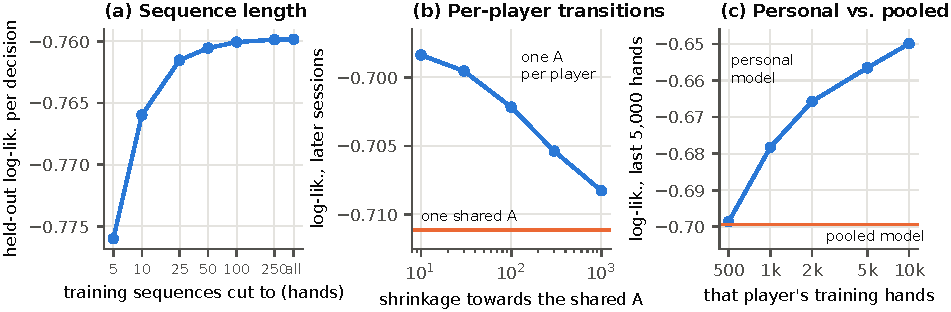
\includegraphics[width=\linewidth]{../figures/fig_ablation.pdf}
\caption{(a) Held-out log-likelihood when training sessions are cut into pieces of a given length. (b) Shared emissions with one transition matrix per player, for different amounts of shrinkage. (c) A personal four-state HMM trained on a player's first $n$ hands against the pooled model, on that player's last 5{,}000 hands (31 high-volume players).}
\label{fig:ablation}
\end{figure}

\begin{table}[h]
\caption{Alphabet and context, $K=4$. All models are scored on the same task: one-step-ahead log-probability of fold / check-call / raise on new players. $V$ is Cram\'er's $V$ between decoded state and position (0 = unrelated).}
\label{tab:abl}
\centering\small
\begin{tabular}{lrrrr}
\toprule
 & Parameters & $K=1$ & $K=4$ & $V$\\
\midrule
3 symbols, no context & 23 & $-0.754$ & $-0.728$ & 0.003\\
8 symbols, no context & 43 & $-0.754$ & $-0.733$ & 0.009\\
3 symbols, with context & 95 & $-0.649$ & $\mathbf{-0.609}$ & 0.005\\
8 symbols, with context (main) & 295 & $-0.649$ & $-0.615$ & 0.009\\
\bottomrule
\end{tabular}
\end{table}

\begin{table}[h]
\caption{Event study on held-out sessions: change in VPIP after a big loss minus change after a big win, in percentage points, with 95\% intervals from a bootstrap over players.}
\label{tab:sub}
\centering\small
\begin{tabular}{lrr}
\toprule
Subset & Big losses & Loss minus win\\
\midrule
All held-out events & 13{,}957 & $+1.04$ $[0.78,1.31]$\\
Stake \$0.25 & 4{,}187 & $+1.41$ $[1.00,1.84]$\\
Stakes \$4 to \$10 & 9{,}770 & $+0.88$ $[0.57,1.19]$\\
Sessions on 1--2 tables & 820 & $+1.49$ $[0.33,2.63]$\\
Sessions on 3 or more tables & 13{,}137 & $+1.01$ $[0.76,1.29]$\\
Players with fewer than 3{,}000 hands & 1{,}702 & $+1.40$ $[0.62,2.20]$\\
Players with 3{,}000 hands or more & 12{,}255 & $+0.99$ $[0.74,1.26]$\\
Threshold 30\,bb & 21{,}233 & $+0.95$ $[0.71,1.18]$\\
Threshold 100\,bb & 7{,}922 & $+1.09$ $[0.76,1.43]$\\
\bottomrule
\end{tabular}
\end{table}

\begin{table}[h]
\caption{Pooled input-output HMM: probability of \emph{staying} in the current state at the next hand, by input, with 95\% bootstrap intervals (200 resamples of training players) for the after-loss row.}
\label{tab:io}
\centering\small
\begin{tabular}{lrrrr}
\toprule
 & S1 & S2 & S3 & S4\\
\midrule
No event & 0.9991 & 0.9985 & 0.9987 & 0.9974\\
After a big win & 0.9977 & 0.9943 & 0.9980 & 0.9939\\
After a big loss & 0.9955 & 0.9944 & 0.9859 & 0.9905\\
\quad 95\% interval & [0.989, 0.999] & [0.980, 0.998] & [0.971, 0.994] & [0.978, 0.997]\\
\bottomrule
\end{tabular}
\end{table}

\begin{table}[h]
\caption{Models with per-player parameters: test log-likelihood per decision (each player's last 30\% of hands; 2.74M decisions).}
\label{tab:personal}
\centering\small\setlength{\tabcolsep}{3.5pt}
\begin{tabular}{lrr}
\toprule
Model & 8 symbols & 3 symbols\\
\midrule
Pooled, no hidden state & $-0.8439$ & $-0.6359$\\
Pooled HMM, $K=4$ / $K=8$ & $-0.7511$ / $-0.7359$ & \\
Per-player table, no hidden state & $-0.6986$ & $-0.5851$\\
\quad + second mode, weak prior ($\kappa_2=20$): no switching / HMM & $-0.7021$ / $-0.7014$ & $-0.5862$ / $-0.5861$\\
\quad + second mode, strong prior ($\kappa_2=320$): no switching / HMM & $-0.6974$ / $-0.6972$ & $-0.5849$ / $-0.5852$\\
\shiftrows
\bottomrule
\end{tabular}
\end{table}

\begin{table}[h]
\caption{Negative control. Personal HMMs with contexts, five-fold cross-validation over sessions; change in log-likelihood per decision relative to $K=1$.}
\label{tab:pluribus}
\centering\small
\begin{tabular}{lrrrrr}
\toprule
Player & Hands & $K=1$ & $K=2$ & $K=3$ & $K=4$\\
\midrule
Pluribus (bot) & 10{,}000 & $-0.6953$ & $-0.0001$ & $-0.0002$ & $-0.0004$\\
MrBlue & 9{,}121 & $-0.7041$ & $-0.0001$ & $-0.0003$ & $-0.0004$\\
MrOrange & 7{,}512 & $-0.6161$ & $-0.0007$ & $-0.0005$ & $-0.0006$\\
Bill & 6{,}713 & $-0.6537$ & $+0.0060$ & $+0.0010$ & $-0.0006$\\
MrPink & 6{,}055 & $-0.6401$ & $-0.0002$ & $-0.0004$ & $-0.0006$\\
Eddie & 5{,}510 & $-0.6864$ & $-0.0011$ & $-0.0013$ & $-0.0007$\\
MrWhite & 4{,}483 & $-0.6555$ & $-0.0003$ & $-0.0005$ & $-0.0008$\\
\midrule
40 PartyPoker players & 10{,}000 each & \multicolumn{4}{l}{best $K>1$: median $-0.0001$; better than $K=1$ for 28\%}\\
\bottomrule
\end{tabular}
\end{table}


\end{document}
